%
% General structure for the revdetua class:
%

\documentclass[...]{revdetua}
\usepackage{graphicx}
%
% Valid options are:
%
%   longpaper --------- \part and \tableofcontents defined
%   shortpaper -------- \part and \tableofcontents not defined (default)
%
%   english ----------- main language is English (default)
%   portugues --------- main language is Portuguese
%
%   draft ------------- draft version
%   final ------------- final version (default)
%
%   times ------------- use times (postscript) fonts for text
%
%   mirror ------------ prints a mirror image of the paper (with dvips)
%
%   visiblelabels ----- \SL, \SN, \SP, \EL, \EN, etc. defined
%   invisiblelabels --- \SL, \SN, \SP, \EL, \EN, etc. not defined (default)
%
% Note: the final version should use the times fonts
% Note: the really final version should also use the mirror option
%




\begin{document}

\Header{1}{1}{Dezembro}{2020}{1}
% Note: the month must be in Portuguese

\title{Exhaustive search application for the maximum clique problem}
\author{Rodrigo Ferreira} % or \author{... \and ...}
\maketitle

\begin{resumo}% Note: in Portuguese
	Este artigo começa por contextualizar conceitos essenciais ao tema do problema, como o conceito de grafo, nós, arestas, sub-grafo e sub-grafo completo. Passa então descrever o problema em questão. Depois de estabelecidas tais bases, explica o conceito de algoritmos de força bruta e em particular, pesquisa exaustiva. As suas características, vantagens, desvantagens, e como se encaixa no problema em questão, assim como uma avaliação dos resultados obtidos para o problema de clique máximo.
\end{resumo}

\begin{abstract}% Note: in English
  This paper starts out by contextualizing important concepts, essential to understand its theme, like graphs, nodes, edges, subgraphs and complete subgraphs. Afterwards, the problem at hand is described. When the basic concepts and the problem have been explained, we move on to the topic of brute force algorithms, and exhaustive search in particular. Its characteristics, advantages, disadvantages, how it fits into this theme, as well as an evaluation of its results when applied to the max clique problem.
\end{abstract}
\section{Introduction}
\subsection{Fundamental concepts}
We can’t discuss the max clique problem without first establishing some key concepts regarding graphs.
\begin{itemize}
\item Graphs are structures composed of 2 sets, a set V, of nodes, and a set E of edges (we are always talking about undirected graphs in this paper) \cite{graph}.
\item Nodes, vertices, or points are the fundamental unit of which graphs are formed, in a graph diagram they are objects usually represented by a circle with a label  \cite{graph}.
\item Edges are the other basic unit of which graphs are made of. Each edge has two vertices as endpoints, edges can be directed or undirected, but in the case at hand, they are always undirected which means $(i,j)$ implies $(j,i)$ and vice versa, as opposed to directed edges (arcs) where we may have only $(i,j)$ or $(j,i)$ . In a graph diagram, edges are usually represented by a line uniting two nodes  \cite{graph}.
\item A subgraph is a graph formed from a subset of nodes and edges of another graph\cite{subgraph}.
\item A complete graph/subgraph is a subgraph that has an edge connecting every pair of its  vertices\cite{completegraph}.
\end{itemize}
\subsection{The problem}
Now that the basic concepts relevant to the problem have been estabilished, we can move on to describing the problem itself.\par
The maximum clique of a graph $G$ is a complete subgraph $G'$ such that no other complete subgraph in $G$ has cardinality higher than $\#G'$, as demonstrated in the following image, where the subgraph containing the vertices ${\{2,3,4,6\}}$ represents the max clique.\par
\begin{center}
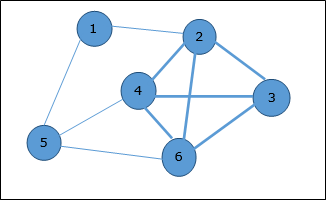
\includegraphics[scale=0.8]{max_clique_example}
\end{center}
\label{Example of a max clique of a graph}
It's a simple description to a difficult problem, the task of finding whether there is a clique of a given size in a graph (the clique problem) is NP-complete \cite{wikiclique}, meaning it's in the NP class (solved by a non-deterministic Turing machine in polynomial time) and also that every problem in NP can be reduced to the clique problem in polynomial time.\par 
And thus, if an algorithm is found to solve the clique problem in polynomial time with a deterministic Turing machine, all problems in NP are suddenly also solved \cite{wikinp}. 
\section{The approach}
\subsection{Brute force algorithms}
Brute force algorithms use a straightforward approach to solving problems taking advantage of a machine's computing power, over that of a human being.\par
It is usually directly based on the problem statement and definitions of the concepts involved \cite{brute}. 
\subsection{Exhaustive search}
Exhaustive search is a brute force approach to combinatorial problems.
It generates all candidate answers, and then checks each of them to confirm their validity, returning the best \cite{exh}.\par
This approach, simple and effective, always returning a solution if there is one, can tackle most problems we can think of while usually requiring a very simple implementation, but there's a caveat, it's extremely inefficient due to its blind "try everything" approach.\par And thus, it's only advised for very small instances of the problems it can solve, due to its difficulties for bigger instances, as the number of possible candidates grows because of the combinatorial nature of the problems it tackles.

\section{The algorithm}
A quality of exhaustive search algorithms is that the code is very simple.\par
It only takes a small function, which will be briefly described, to get the maximum clique/s from a set of nodes N and a set of edges M.\par
First, we notice that the maximum clique for a graph $G$ with $1<=N$ vertices must have a cardinality between $1$ and $\#N$, $1$ assuming there are no edges, and $\#N$ assuming $G$ is a complete graph, and thus, a clique.\par
Once we become aware of this, we can make a cycle where we generate all combinations (could be permutations but it would be useless because we're using undirected graphs, i.e. $(i,j)=(j,i)$) of vertices with size $1$ to $N$.\par
When we get all these combinations, we go one by one, and test if indeed there exists an edge for every pair of vertices in said combination, if it does constitute a clique, we append it to a structure (dictionary where the key represents the cardinality of the solutions it maps to, and the value is a list of sets of nodes with that cardinality) containing all solutions, and update another variable, $max$, to keep track of the cardinality of the best solution found so far, otherwise we ignore it.\par
Finally, when the program has run its course for all combinations of size $1$ to $N$, we obtain the maximum cliques by accessing our dictionary with $max$ as key.
	
\subsection{Complexity}
It's easy to see, given the algorithm's description, that its complexity depends only on the size of the set of vertices $N$, because all combinations are tested, and thus all possible edges are tested, whether they exist in the graph or not.\par
Due to the fact that the program's complexity is solely based on the size of the set of vertices, all graphs with the same $\#N$ have the same number of basic operations.\par
Another consequence of applying exhaustive search is that the worst, average and best case are all the same for every instance of the problem as it checks every possibility regardless. \par
The complexity is given by the following formula, which is quite intuitive once the algorithm has been analysed, basically we generate all combinations of size $1$ to $\#N$ and check every pair of vertices in all combinations, thus: 
$$\sum_{i=1}^{n}{{n}\choose{i}}{{i}\choose{2}}=2^{(n-3)}(n-1)n$$
This means that our algorithm is in $O(2^{(n-3)}(n-1)n)$, making it an exponential algorithm. 
\subsection{Testing for bigger instances}
\subsubsection{Basic operation count}
As we are working with an algorithm with complexity $2^{(n-3)}(n-1)n$, the amount of basic operations (an instruction in the innermost loop) executed grows explosively as $\#N$ increases.\par This can be observed in the following image.
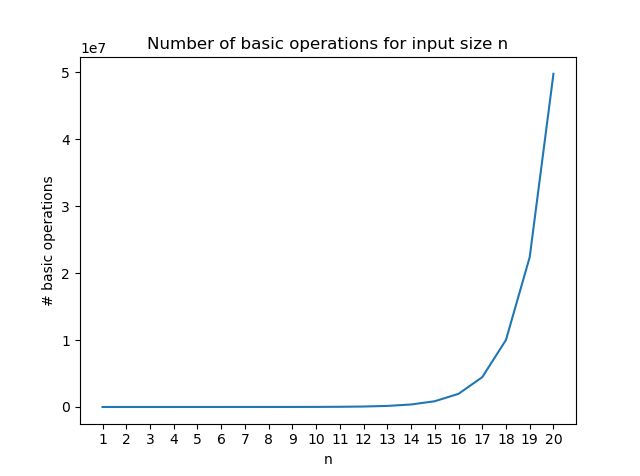
\includegraphics[scale=0.5]{basic_ops.png}
\subsubsection{Execution time}
As a consequence of the number of basic operations growing by such a factor as we increase $\#N$, the executing time will also grow very fast as well, as is demonstrated in the following graphic.

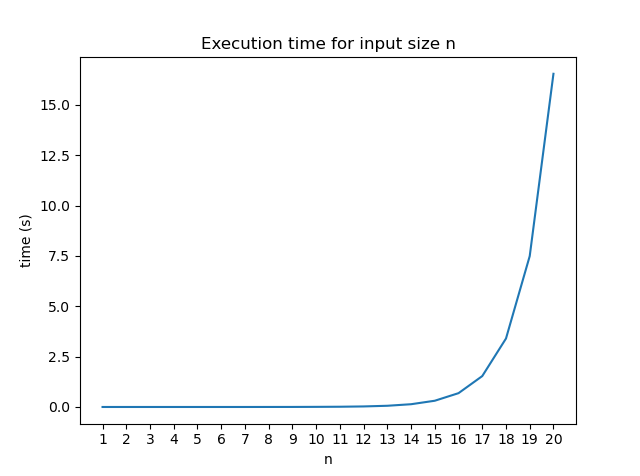
\includegraphics[scale=0.5]{exe_time.png}
\subsubsection{Solutions and total configurations}
On our complexity formula it's clear the sheer amount of configurations generated for each $\#N$ is very big (given by $\sum_{i=1}^{n}{{n}\choose{i}}$) and it's unrealistic to assume the number of solutions can accompany such growth, thus our ratio $\frac{\#solutions}{\#configurations}$ will decrease as $\#N$ grows bigger, as the following image shows.
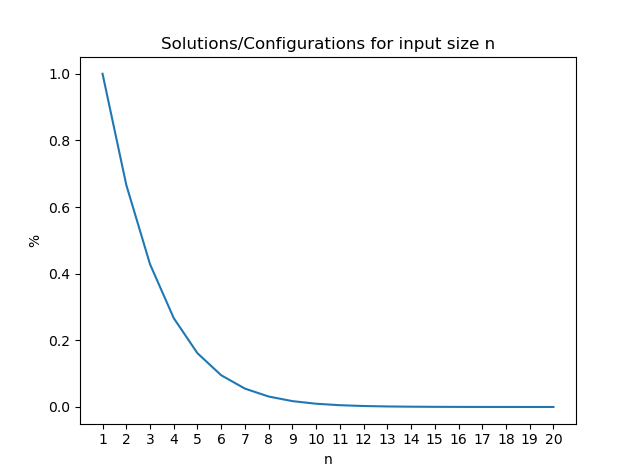
\includegraphics[scale=0.5]{solconfig.png}
\subsection{Comparing results}
The results seem to coincide with our previous complexity analysis as the number of basic operations counted within the code provides the exact same value as our complexity formula.\par
And the execution time graphic is also very similar to the plotting of ${2^{(n-3)}(n-1)n}$.
\subsection{Estimating running time for bigger instances}
With our previous results we can pick an $\#N$, get its number of basic operations and executing time, and get $$X=\frac{basic\ operations}{executing\ time}$$ where $X$ gives us an estimate of the basic operations done per second, for a huge instance size $j$, we simply have to calculate its number of operations using  our formula $2^{(n-3)}(n-1)n$ with $n=j$, we can then multiply that number of operations with $X$ to get an estimate of the running time for an instance of size $j$, though this is only a rough estimate.

\section{Conclusions}
This example was effective at showing the pros and cons of exhaustive search algorithms, we managed to make a very simple program, that works very well for smaller instances of our problem, but scales very poorly, leaving us to wait for an answer, which might take an unimaginable amount of time and huge computational resources to achieve.
%\section{References}


%[1]\url{https://en.wikipedia.org/wiki/Clique_(graph_theory)}
%[2]\url{https://en.wikipedia.org/wiki/NP-completeness}\par
%\
%[3]	A. Levitin, Introduction to the Design and Analysis of Algorithms, 3rd Ed., Pearson, Chapter 3,pp.97-98, 2012\par
%\
%[4]	A. Levitin, Introduction to the Design and Analysis of Algorithms, 3rd Ed., Pearson, Chapter 3,pp.115, 2012

\bibliography{bibliografia}
\end{document}
